Para el analisis de los resultados es importante notar que en el eje y estan los tiempos de ejecucion en microsegundos
y en el eje x se tiene el largo de las cadenas de entrada, estos graficos estan dentro del archivo de la tarea, el archivo
el archivo en cuestion se llama graficos.ipynb, las graficas no son generadas de manera automatica por lo que estos son los resultados
de un promedio de 3 pruebas para cada datasets, favor de observar el codigo y en caso de replicar el experimento identificar los
datos a cambiar para asi poder ver sus respectivas graficas, el programa esta hecho en jupyther y es muy intuitivo de usar para cambiar
los resultados experimentales puede ver el codigo aca \url{https://github.com/Daspssj/Tarea2_3/blob/main/graficos.ipynb}, para 
generar los datos en caso de querer replicar el trabajo favor de compilar y ejecutar el archivo de Crear\_datasets.cpp 
\url{https://github.com/Daspssj/Tarea2_3/blob/main/Crear_datasets.cpp} y para generar sus propios resultados se tiene que compliar
y ejecutar el archivo de Algoritmos.cpp \url{https://github.com/Daspssj/Tarea2_3/blob/main/Algoritmos.cpp} el programa implementado es
bastante amigable con el ususario por lo que no sera dificil usarla, a continuacion se presentan los resultados obtenidos de las pruebas realizadas:

\begin{figure}[H]
    \centering
    \begin{minipage}[t]{0.5\textwidth}
        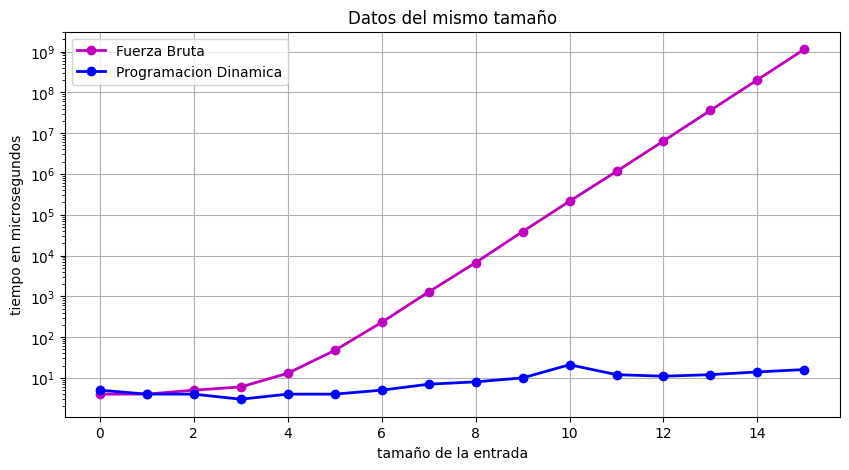
\includegraphics[width=\textwidth]{images/mismotananio.png}
    \end{minipage}%
    \begin{minipage}[t]{0.5\textwidth}
        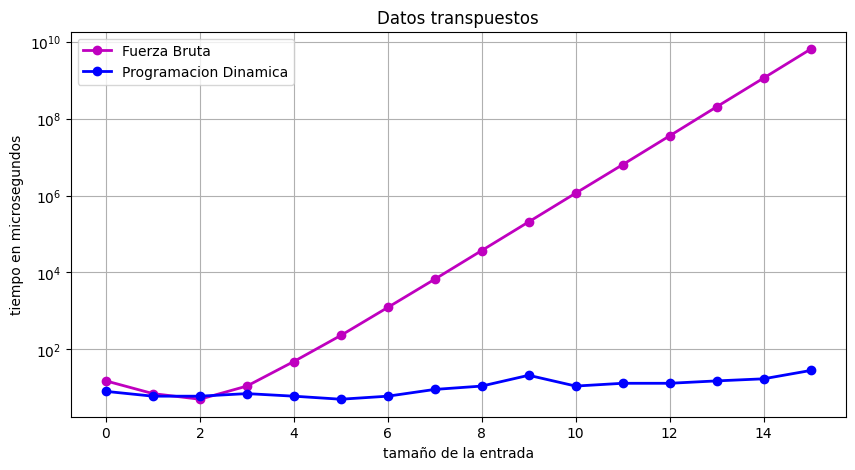
\includegraphics[width=\textwidth]{images/transpuesto.png}   \end{minipage}%
    \caption{Tiempos de ejecucion vs largo de las cadenas}
    \label{fig:Tiempos de ejecucion vs largo de las cadenas}
\end{figure}

\begin{figure}[H]
    \centering
    \begin{minipage}[t]{0.5\textwidth}
        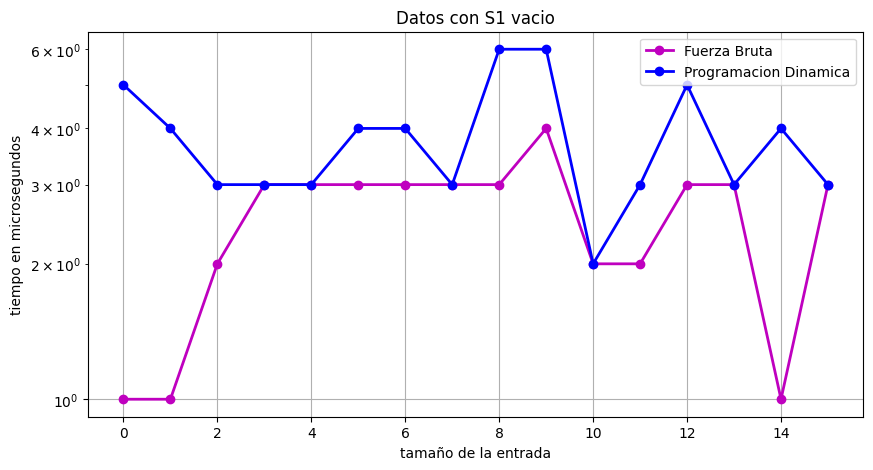
\includegraphics[width=\textwidth]{images/s1vacio.png}
    \end{minipage}%
    \begin{minipage}[t]{0.5\textwidth}
        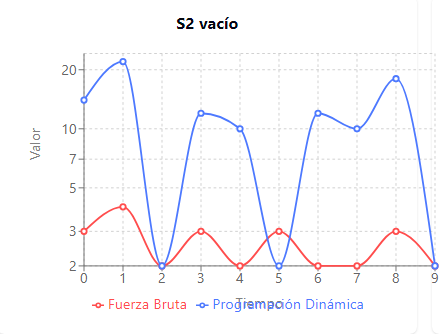
\includegraphics[width=\textwidth]{images/s2vacio.png}   \end{minipage}%
    \caption{Tiempos de ejecucion vs largo de las cadenas}
    \label{fig:Tiempos de ejecucion vs largo de las cadenas}
\end{figure}

\begin{figure}[H]
    \centering
    \begin{minipage}[t]{0.5\textwidth}
        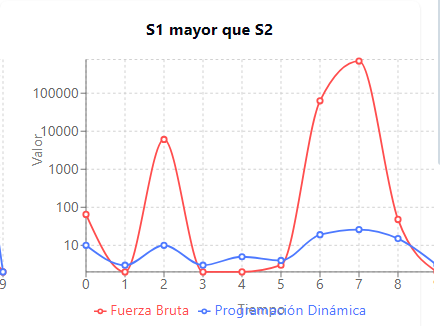
\includegraphics[width=\textwidth]{images/s1mayor.png}
    \end{minipage}%
    \begin{minipage}[t]{0.5\textwidth}
        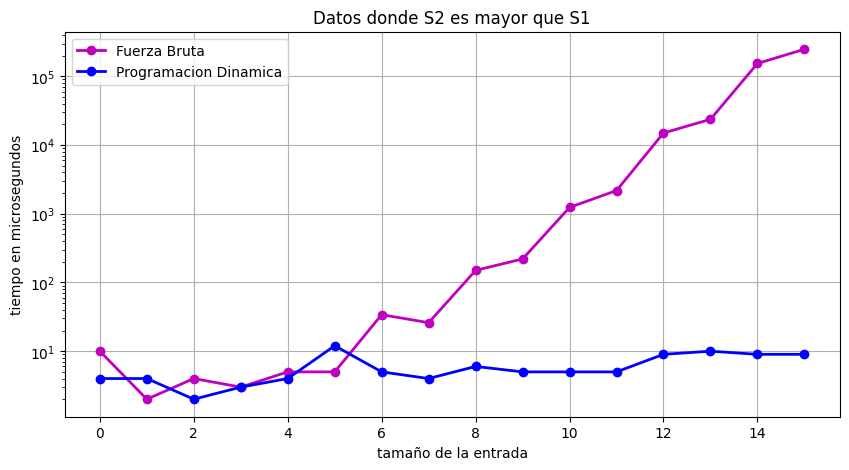
\includegraphics[width=\textwidth]{images/s1menor.png}   \end{minipage}%
    \caption{Tiempos de ejecucion vs largo de las cadenas}
    \label{fig:Tiempos de ejecucion vs largo de las cadenas}
\end{figure}


Como podemos observar en los primeros 2 graficos correspondientes a la figura 1 se puede observar que los tiempos de ejecucion de cada algoritmo 
son muy distintos entre si y esto se debe a las complejidades temporales de los algoritmos, se puede ver que el agoritmo de fuerza bruta 
crece de manera exponencial mientras que programacion dinamica se mantiene en un rango de valores aceptable, luego para los algunos de los strings
vacios se ve que Fuerza bruta tiene un tiempo de ejecucion mas bajo que el de programacion dinamica aunque no mucho igualmente se puede
ver en los graficos de la figura 2 y por ultimo para los strings de distinto tamaño se puede ver que el algoritmo de fuerza bruta tiene un tiempo 
de ejecucion mas alto que el de programacion dinamica, sin embargo estos tiempos no son tan altos como en el caso de los strings de
mismo tamaño ya que solo se transpone una cadena, esto quiere decir que no se tiene que recorrer todas las posibles combinaciones
entre insertar, eliminar, sustituir o transponer.


Por otro lado tenemos el uso de memoria de los algortimos, donde el algoritmo de fuerza bruta tiene un uso de memoria de $O(n)$, lo que significa que
su uso de memoria es lineal en donde $n$ es el tamaño de la cadena de entrada, por otro lado tenemos el algoritmo de programacion dinamica
el cual su uso de memoria es el tamaño en bytes de la matriz que se crea para almacenar los resultados de las subcadenas, por lo que su uso de memoria
es de $O(n \times m)$ donde $n$ y $m$ son los tamaños de las cadanas de entrada.


Nota: Es importante tener en cuenta el uso del cache para el primer resultado de fuerza bruta y programacion dinamica, ya que
se tiene que en algunos casos el primer tiempo de ejecucion de los algoritmos son raramente mas altos que los demas primeros datos.